\chapter{Gaussian distribution}
In this chapter, the basic properties of Gaussian distributions are given, with special attention in regard to the \textbf{multivariate Gaussian distribution}. As the name suggests, \textbf{Gaussian processes} are in fact based on these multivariate distributions, exploiting properties that will be shown throughout the chapter.\\
The sources used in writing the chapter are \cite{gut_intermediate_2009}, \cite{wilkinson_introduction_2020}, \cite{murphy_probabilistic_2022}.


\begin{textblock*}{0.64\textwidth}(3.5cm+0.36\textwidth,18.5cm)
\epigraph{At a purely formal level, one could call probability theory the study of measure spaces with total measure one, but that would be like calling number theory the study of strings of digits which terminate.}{Terence Tao}
\end{textblock*}

\newpage

%%%%%%%%%%%%%%%%%%%%%%%%%%%%%%%%%%%
%%%%%% GAUSSIANA UNIVARIATA
%%%%%%%%%%%%%%%%%%%%%%%%%%%%%%%%%%%


\section{Univariate Gaussian distribution}
\begin{defi}[Univariate Gaussian distribution]
    The \textbf{univariate Gaussian distribution} is a continuous probability distribution. \\
    Given $Y\sim \mathcal{N}(\mu, \sigma^2)$, its probability density function is expressed as:
    \[f_Y(y) = \frac{1}{\sqrt{2\pi \sigma^2}} \text{exp}\bigg\{-\frac{1}{2}\frac{(y-\mu)^2}{\sigma^2}\bigg\}.\]
\end{defi}


%%%%%%%%%%%%%%%%%%%%%%%%%%%%%%%%%%%
%%%%%% IMMAGINI GAUSSIANA
%%%%%%%%%%%%%%%%%%%%%%%%%%%%%%%%%%%
\begin{figure}[h]
\centering
\begin{subfigure}{.5\textwidth}
  \centering
  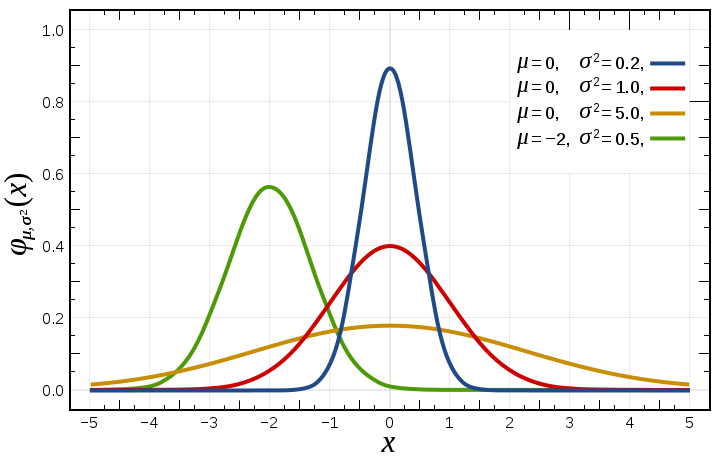
\includegraphics[width=\linewidth]{images/Gaussiane/PDFNormalDistribution.png}
  \caption{Probability density}
  \label{fig:sub1}
\end{subfigure}%
\begin{subfigure}{.5\textwidth}
  \centering
  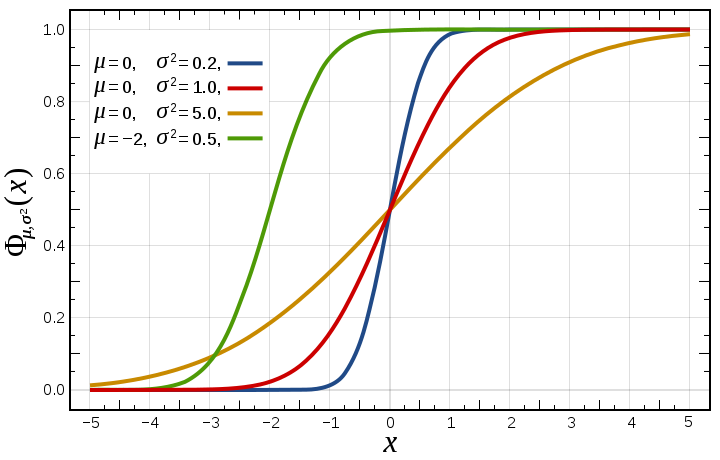
\includegraphics[width=\linewidth]{images/Gaussiane/CDFNormalDistribution.png}
  \caption{Distribution function}
  \label{fig:sub2}
\end{subfigure}
\caption{Distribution function and probability density of a standard normal distribution \cite{wikiNormalDistribution}.}
\label{fig:gaussian}
\end{figure}



\begin{oss} \label{normal decomposition}
Given $Z\sim \mathcal{N}(0,1)$ it follows:  $Y=\mu + \sigma Z\sim \mathcal{N}(\mu,\sigma^2)$.
\end{oss}

\begin{oss}
    Informally speaking, the Gaussian distribution is "convenient" mathematically because of its properties:
\begin{itemize}
    \item the normal distribution has two parameters that are easy to interpret: the mean and the variance;
    \item the normal distribution is closed under linear operations;
    \item the normal distribution is closed by marginalization and conditioning (see the proposition \ref{marginale-condizionata});
    \item at equal mean and variance, the normal distribution has maximum entropy;
    \item from \textbf{central limit theorem}, the normal distribution is the limit of a sum of random variables; 
    \item the normal distribution has a simple mathematical form that facilitates its implementation.
\end{itemize}
\end{oss}


\newpage


%%%%%%%%%%%%%%%%%%%%%%%%%%%%%%%%%%%
%%%%%% GAUSSIANA MULTIVARIATA
%%%%%%%%%%%%%%%%%%%%%%%%%%%%%%%%%%%
\section{Multivariate Gaussian distribution}


The multivariate Gaussian distribution is a generalization of the normal (univariate) distribution.



\begin{defi}[Multivariate Gaussian distribution] An $n$-dimensional $\mathbf{X}$-vector of random variables is said to be normal (\textbf{multivariate normal}) if and only if $\forall \mathbf{a} in \mathbb{R}^n$ the random variable $\mathbf{a}^\text{T}\mathbf{X}$ is a normal distribution.  
    The density\footnote{In the generalized case it is not possible to define the density of the multivariate Gaussian distribution. As will be shown later, in Gaussian processes the density is not as important as the covariance matrix and the mean vector.} of a \textbf{multivariate Gaussian distribution} is expressed as
\[f_{\mathbf{X}}(\mathbf{x})=\frac{1}{(2\pi)^{\sfrac{n}{2}}  \text{det}(\bm{\Sigma})^{\sfrac{1}{2}}} \text{ exp}\left[-\frac{1}{2}(\bm{x}-\bm{\mu})^\text{T}\bm{\Sigma}^{-1}(\bm{x}-\bm{\mu})\right]
\]\end{defi}
where $\bm{\mu}=\mathbb{E}[\bm{X}]\in \mathbb{R}^n$ is the  \textit{mean vector}, $\bm{\Sigma}=\text{Cov}[\bm{X}]$ is a $n\times n$ matrix called \textit{covariance matrix}, defined as:
\[\begin{split}
\text{Cov}[\bm{X}] &= \mathbb{E}\left[(\bm{X}-\mathbb{E}[\bm{X}])(\bm{X}-\mathbb{E}[\bm{X}])^\text{T} \right]\\
 & = \begin{pmatrix}
    \mathbb{V}[X_1] & \text{Cov}[X_1,X_2] & \dots & \text{Cov}[X_1,X_n]\\
    \text{Cov}[X_2,X_1] & \mathbb{V}[X_2] & \dots & \text{Cov}[X_2,X_n]\\
    \vdots & \vdots & \ddots & \vdots\\
    \text{Cov}[X_n,X_1] & \text{Cov}[X_n,X_2] & \dots & \mathbb{V}[X_n]
    \end{pmatrix}
\end{split}
\]
where:
\[ \text{Cov}[X_i,X_j]=\mathbb{E}[(X_i-\mathbb{E}[X_i])(X_j-\mathbb{E}[X_j])] = \mathbb{E}[X_iX_j]-\mathbb{E}[X_i]\mathbb{E}[X_j]  \]
\[ \mathbb{V}[X_i]=\text{Cov}[X_i, X_i]. \]


\begin{oss}\label{ossGaussianaMultivariata}
    The covariance matrix is symmetrical and semidefinite positive, i.e., $\forall \mathbf{a} \in \mathbb{R}^n$ one has $\mathbf{a}^\text{T} \mathbf{a}\geq 0$.
\end{oss}


%%%%%%%%%%%%%%%%%%%%%%%%%%%%%%%%%%%
%%%%%% COROLLARIO DEFINIZIONE
%%%%%%%%%%%%%%%%%%%%%%%%%%%%%%%%%%%
\begin{cor}
    Given $\mathbf{X}$ a multivariate normal vector, from the definition of multivariate Gaussian distribution follow immediately:
\begin{enumerate}
    \item each component of $\mathbf{X}$ is a Gaussian random variable;
    \item $\sum_{i=1}^{n} a_iX_i$ is a Gaussian random variable $\forall a_i\in \mathbb{R}$;
    \item If the components of $\mathbf{X}$ are independent Gaussian random variables, then $\mathbf{X}$ is a multivariate normal vector.
\end{enumerate}
\end{cor}

\begin{oss}
    The third point of the previous corollary does not hold if the components are not independent. For example: $X\sim \mathcal{N}(0,1)$, $Z\indep X$, $\mathbb{P}(Z=1)=\mathbb{P}(Z=-1)=\sfrac{1}{2}$. It is easily seen that $Y=ZX$ is not independent of $X$ and $\begin{pmatrix}
X\\
Y
\end{pmatrix}$ is not multivariate normal.
\end{oss}

\newpage


%%%%%%%%%%%%%%%%%%%%%%%%%%%%%%%%%%%
%%%%%% PROPOSIZIONE
%%%%%%%%%%%%%%%%%%%%%%%%%%%%%%%%%%%
Of critical importance is the next proposition. The proof is omitted because it consists of lengthy calculations that are outside the scope of the paper. For the proof, please refer to \cite{murphy_probabilistic_2022}.
\begin{prop}[Marginal and conditional distribution] \label{marginale-condizionata}
Let $\bm{Y}=\begin{pmatrix}\bm{y}_1 \\ \bm{y}_2\end{pmatrix}$ Gaussian multivariate vector where:
\[
\bm{\mu}=\begin{pmatrix}\bm{\mu}_1\\ \bm{\mu}_2\end{pmatrix}\quad
 \bm{\Sigma}=\begin{pmatrix}\bm{\Sigma}_{11}&\bm{\Sigma}_{12}\\ \bm{\Sigma}_{21}&\bm{\Sigma}_{22}\end{pmatrix}\quad \bm{\Lambda}=\bm{\Sigma}^{-1}=\begin{pmatrix}\bm{\Lambda}_{11}&\bm{\Lambda}_{12}\\\bm{\Lambda}_{21}&\bm{\Lambda}_{22}\end{pmatrix}
\]
Then the marginal distributions are:
\[
\bm{y}_1\sim \mathcal{N}(\bm{\mu}_1, \bm{\Sigma}_{11}) \qquad \bm{y}_2\sim \mathcal{N}(\bm{\mu}_2, \bm{\Sigma}_{22})
\]
While conditional distributions are:
\[
\bm{y}_1 | \bm{y}_2 \sim \mathcal{N}(\bm{\mu}_{1|2}, \bm{\Sigma}_{1|2}) \qquad
\def\arraystretch{1.4}
\begin{array}{l}
    \bm{\mu}_{1|2}        =\bm{\mu}_1+\bm{\Sigma}_{12}\bm{\Sigma}_{22}^{-1}(\bm{y}_2-\bm{\mu}_2)\\
    \bm{\Sigma}_{1|2}=\bm{\Sigma}_{11}-\bm{\Sigma}_{12}\bm{\Sigma}_{22}^{-1}\bm{\Sigma}_{21}=\bm{\Lambda}_{11}^{-1}
\end{array}
\]

\[
\bm{y}_2 | \bm{y}_1 \sim \mathcal{N}(\bm{\mu}_{2|1}, \bm{\Sigma}_{2|1})
\qquad
\def\arraystretch{1.4}
\begin{array}{l}
    \bm{\mu}_{2|1}        =\bm{\mu}_2+\bm{\Sigma}_{21}\bm{\Sigma}_{11}^{-1}(\bm{y}_1-\bm{\mu}_1)\\
    \bm{\Sigma}_{2|1}=\bm{\Sigma}_{22}-\bm{\Sigma}_{21}\bm{\Sigma}_{11}^{-1}\bm{\Sigma}_{12}=\bm{\Lambda}_{22}^{-1}
\end{array}
\]
\end{prop}

\newpage

%%%%%%%%%%%%%%%%%%%%%%%%%%%%%%%%%%%
%%%%%% CORRELAZIONE VETTORI
%%%%%%%%%%%%%%%%%%%%%%%%%%%%%%%%%%%
\section{Correlation for multivariate vectors} \label{sezioneCorrelazione}


\begin{defi}[Pearson's correlation index]
The \textbf{Pearson's correlation index} between two random variables is an index expressing a linearity relationship between them. It is expressed as:
\[ \rho_{XY}=\frac{\text{Cov}[X,Y]}{\sqrt{\mathbb{V}[X]\mathbb{V}[Y]}}.
\]
\end{defi}
\begin{oss}[Meaning of $\rho_{XY}$]
    Because of the Cauchy-Schwarz inequality it holds: $-1\leq \rho_{XY}=1$. There are three main cases: $\rho_{XY}=1$ indicates a perfect positive linear relationship; $\rho_{XY}=-1$ indicates a perfect negative linear relationship; $\rho_{XY}=0$ indicates no linear correlation. 
\end{oss}

The remainder of the chapter will focus on the analysis of bivariate Gaussian vectors and the correlation of their components and then generalize the visual approach to multiple dimensions.

%%%%%%%%%%%%%%%%%%%%%%%%%%%%%%%%%%%
%%%%%% CORRELAZIONE GAUSSIANI
%%%%%%%%%%%%%%%%%%%%%%%%%%%%%%%%%%%
Consider a two-dimensional Gaussian vector: \[\mathbf{Y}=\begin{pmatrix}Y_1\\Y_2\end{pmatrix} \qquad\text{con} \qquad \bm{\mu} = \begin{pmatrix}0\\0\end{pmatrix} \quad \mathbf{\Sigma}=\begin{pmatrix}1&0\\0&1\end{pmatrix}.
\]
Generating points from the distribution of $\mathbf{Y}$ (so each point consists of a two-dimensional vector) yields what is shown in figure \ref{correlazione1}.

%%%%%%%%%IMMAGINE
\begin{figure}[h]
    \centering
    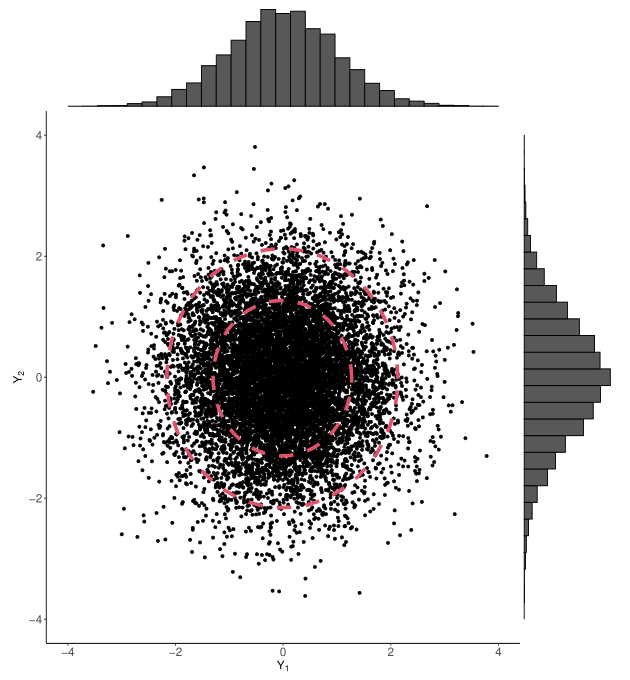
\includegraphics[width=0.65\textwidth]{images/Gaussiane/VettoreBivariatoIndipendenza.png}
    \caption{Point cloud generated by a bivariate Gaussian distribution with uncorrelated components \cite{wilkinson_introduction_2020}.}
    \label{correlazione1}
\end{figure}


\newpage
Note that the point cloud is centered in zero as a consequence of the choice of $\bm{\mu}$. It is easy to compute $\rho_{Y_1,Y_2}=0$ which guarantees the incorrelation of the components of the Gaussian vector. This result can be guessed from the shape of the cloud: given a point in the cloud, knowledge of its $Y_1$ coordinate gives no information about its $Y_2$ coordinate.\\
Now consider $\bm{\mu} = \begin{pmatrix}0\\0\end{pmatrix}$ e $\mathbf{\Sigma}=\begin{pmatrix}1&0.9\\0.9&1\end{pmatrix}$. Generating a cloud of points again yields what is shown in figure \ref{correlazione2}.\\

%%%%%%%%%IMMAGINE
\begin{figure}[h]
    \centering
    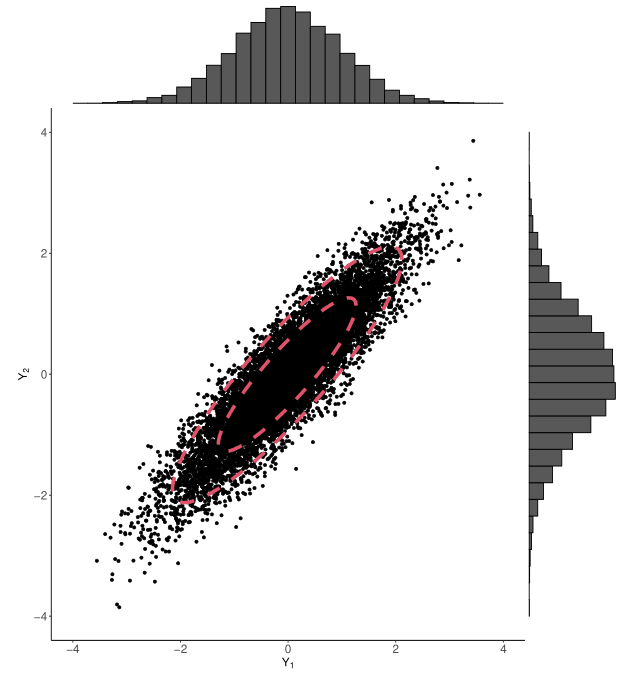
\includegraphics[width=0.7\textwidth]{images/Gaussiane/VettoreBivariatoIndipendenza2.png}
    \caption{Point cloud generated by a bivariate Gaussian distribution with correlated components \cite{wilkinson_introduction_2020}.}
    \label{correlazione2}
\end{figure}

From the shape of the cloud it is now possible to see the correlation between the components of the Gaussian vector. Given a point on the cloud, in fact, the first of the two components gives an approximate idea of the value of the second component (and vice versa): the cloud, to a certain approximation, thickens around a line passing through the origin.\\
The elliptical shape of the cloud is a consequence of the correlation index value: $\rho_{Y_1,Y_2}=0.9$, that is, there is a large linear correlation between the two components.\\

\newpage
Evidently, the elliptical shape becomes more pronounced as the value of the correlation index increases, as can be seen from the figure \ref{correlazione3}, in which $\mathbf{\Sigma}=\begin{pmatrix}1&0.99\\0.99&1\end{pmatrix}$ and thus $\rho_{Y_1,Y_2}=0.99$.

%%%%%%%%%%%IMMAGINE
\begin{figure}[h]
    \centering
    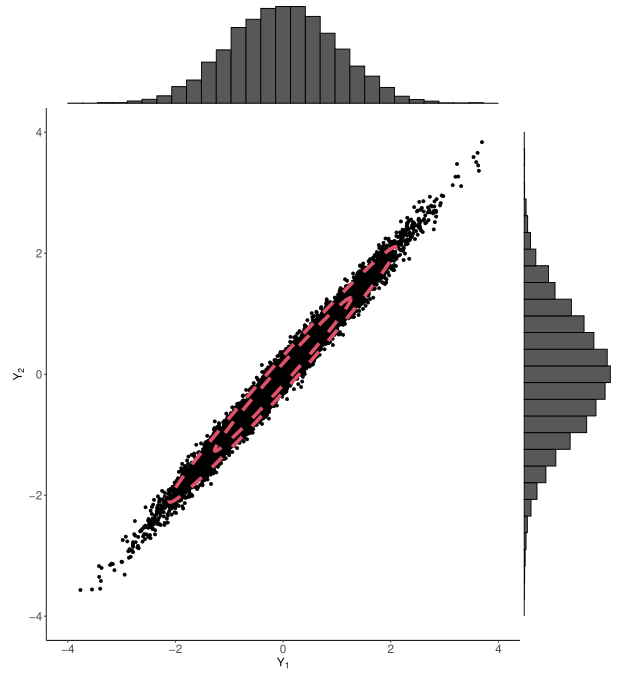
\includegraphics[width=0.7\textwidth]{images/Gaussiane/VettoreBivariatoIndipendenza3.png}
    \caption{Point cloud generated by a bivariate Gaussian distribution with strongly correlated components \cite{wilkinson_introduction_2020}.}
    \label{correlazione3}
\end{figure}



\newpage

In order to generalize to more than two dimensions the visual process of interpreting the correlation between the components of a multivariate Gaussian vector, it is necessary to adopt a different strategy: for each sample (i.e., for each vector) generated by the multivariate Gaussian distribution, the value of the components is plotted in a graph by connecting the respective values by a segment.\\
In figure \ref{correlazione4} the example in two dimensions with $\bm{\mu} = \begin{pmatrix}0\\0\end{pmatrix}$ and $\mathbf{\Sigma}=\begin{pmatrix}1&0.54\\0.54&0.3\end{pmatrix}$. The graph on the left shows the approach used so far; the graph on the right shows for each point on the left graph the value of the first component at index $1$ on the abscissae and the value of the second component at index $2$ on the abscissae.


%%%%%%%%%%%IMMAGINE
\begin{figure}[h]
    \centering
    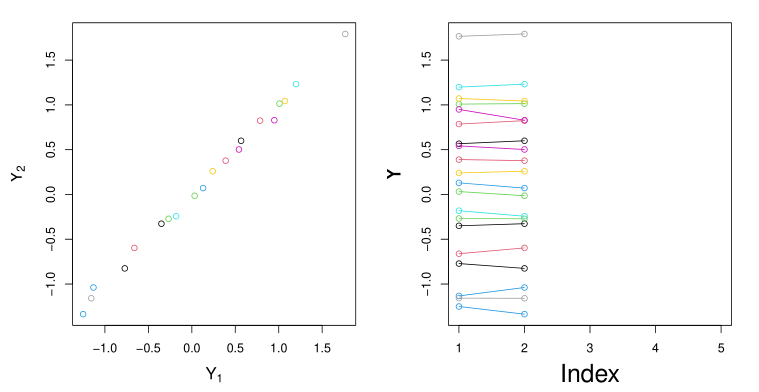
\includegraphics[width=\textwidth]{images/Gaussiane/CorrelazioneMultidimensionale.png}
    \caption{Two different visual approaches to correlation of components of multivariate Gaussian vectors: $n=2$ \cite{wilkinson_introduction_2020}.}
    \label{correlazione4}
\end{figure}


\newpage 

This approach allows generalization to dimensions $n>2$. Let it be now:
\[\bm{\mu}=\bm{0} \qquad\qquad \bm{\Sigma}=\begin{pmatrix}1&0.99&0.98&0.97&0.96\\0.99&1&0.99&0.98&0.97\\0.98&0.99&1&0.99&0.98\\0.97&0.98&0.99&1&0.99\\0.96&0.97&0.98&0.99&1 \end{pmatrix}
\]
Where the components are strongly correlated with each other. We obtain what is shown in the figure \ref{correlazione5}.

%%%%%%%%%%%IMMAGINE
\begin{figure}[h]
    \centering
    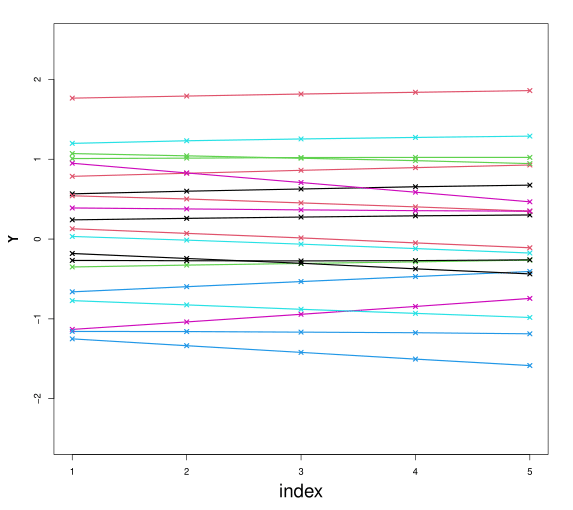
\includegraphics[width=0.7\textwidth]{images/Gaussiane/CorrelazioneMultidimensionale2.png}
    \caption{Visualization using segments of the correlation of components of multivariate Gaussian vectors: $n=5$ \cite{wilkinson_introduction_2020}.}
    \label{correlazione5}
\end{figure}

Being in dimension $n=5$, each sample generated by the Gaussian vector has five components, so when a sample is plotted in the graph it has five points at indices 1, 2, 3, 4, 5.
\newpage

In this case, the strong correlation between the components of the Gaussian vector is reflected in the segment joining the individual points of each sample, as shown in Figure \ref{SegmentCorrelation}.

%%%%%%%%%%%IMMAGINE
\begin{figure}[h]
    \centering
    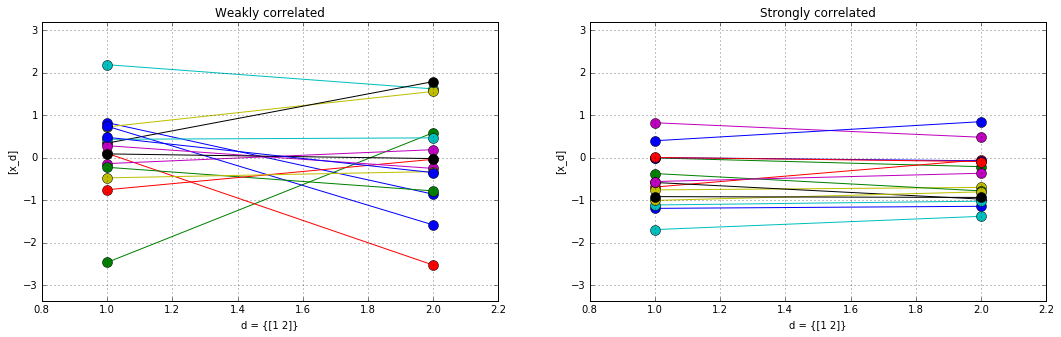
\includegraphics[width=1\textwidth]{images/Gaussiane/CorrelazioneUnidimensionale.png}
    \caption{Weak and strong correlation of components of multivariate Gaussian vectors visualized by segments \cite{damianou_gaussian_2016}.}
    \label{SegmentCorrelation}
\end{figure}

In the case $n=50$ (with null norm vector but omitting the covariance matrix, which continues to have one on the diagonal and values close to one in the other entries), we obtain what is in the figure \ref{correlazione6}.


%%%%%%%%%%%IMMAGINE
\begin{figure}[h]
    \centering
    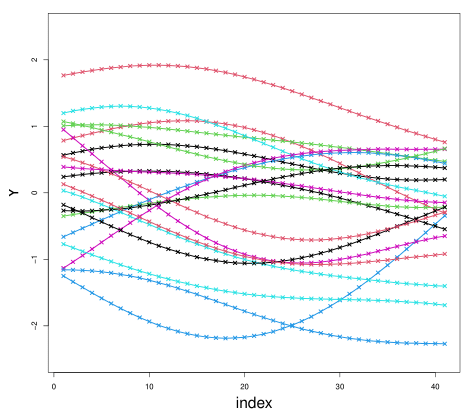
\includegraphics[width=0.7\textwidth]{images/Gaussiane/CorrelazioneMultidimensionale3.png}
    \caption{Visualization by segments of the correlation of components of multivariate Gaussian vectors: $n=50$ \cite{wilkinson_introduction_2020}.}
    \label{correlazione6}
\end{figure}

Notice then that as $n$ increases what obtained begins to resemble a function for each sample generated.\\
From this approach it is possible to interpret Gaussian processes either as functions or as infinite-dimensional multivariate Gaussian distributions ($n=\infty$) with a continuous index (introducing a \textit{mean function} and a \textit{covariance function}). This interpretation will be clarified in the next chapter.